\chapter{Implementation}
% 确定系统功能与架构之后,则需要进行实际的项目开发阶段,在这个阶段会进行开发工具选择,区块链网络设计与搭建,开发平台部署,编码等活动,本节会对这些实施阶段的过程进行简要描述。
In this chapter, activities such as development tool selection, blockchain network design and construction, development platform deployment, and coding are undertaken, and the process of these implementation phases will be briefly described.

\section{Development SDK and Tools Selection}
% 在项目开发中用到的开发工具和SDK都在\tref{Table:toolsused}列出
The development tools and SDKs used in the project development are listed in \tref{Table:toolsused}
\begin{table}[!htb]
\resizebox{\textwidth}{!}{
\begin{tabular}{lll}
\toprule
\textbf{Name}                & \textbf{Usage}                                 & \textbf{Version} \\ \midrule
Virtual Box                  & Run the virtual machine                        & 6.1              \\ \midrule
Vagrant                      & Setup development environment quickly          & 2.2.14           \\ \midrule
Git                          & Project synchronization and collaborative work & 2.30.1           \\ \midrule
Docker                       & Run the blockchain nodes                       & 20.10.8          \\ \midrule
Docker-Compose               & Define Multi-Container                         & 1.29.2           \\ \midrule
Hyper Ledger Fabric          & Build the blockchain network                   & 2.2              \\ \midrule
CouchDB                      & Store the data and state in the blockchain     & 1.4.1            \\ \midrule
Golang                       & Develop the smart contracts                    & 1.16             \\ \midrule
NPM                          & Manage the software and packages               & 6.14.14          \\ \midrule
NodeJS                       & Runtime of the backend application             & 14.17.5          \\ \midrule
Express                      & Server of the backend applicaiton              & 4.17.1           \\ \midrule
MongoDB                      & Storage of insignificant data                  & Online           \\ \midrule
React                        & UI implementation                              & 16.13.1          \\ \midrule
Visual Studio Code           & Use for code                                   & 1.59.1           \\ \midrule
Hyper Ledger Fabric Explorer & Monitor the blockchain                         & 1.1.8           \\
\bottomrule
\end{tabular}
}
\caption{Tools used in project}
\label{Table:toolsused}
\end{table}

\section{Blockchain Network Design}
% 本项目所建立的区块链网络由两个组织组成,每个组织分别拥有两个节点,这两个组织公用一个通道和四个排序节点。网络的结构如\fref{fig:networkarc}所示。
The blockchain network created in this project consists of two organizations, each with two nodes respectively, and these two organizations share a common channel and four raft consensus sorting nodes. The structure of the network is shown in \fref{fig:networkarc}.

\begin{figure}[!htb]
    \centering
    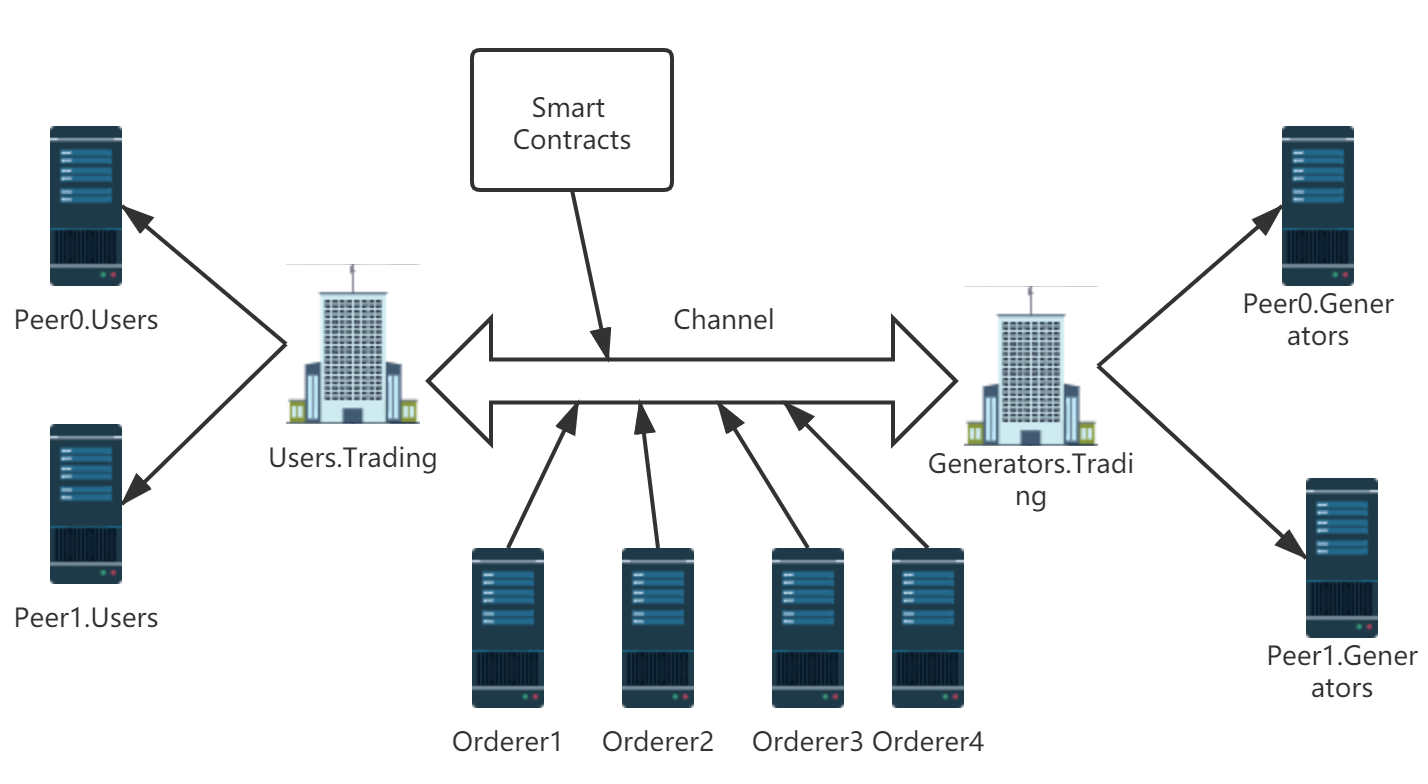
\includegraphics[width=.7 \textwidth]{img/networkarc.png}
    \caption{Blockchain network architecture of the system}
    \label{fig:networkarc}
\end{figure}

% 在设计好网络之后,需要依照Hyper Ledger Fabric的官方文档编写命令脚本对各个组织以及网络节点进行证书,密钥以及创世区块的生成活动,命令运行成功后可以生成项目所建立的区块链网络的基础设施文件,具体的文件结构如\fref{fig:networkfilestructure}.
After designing the network, it is necessary to write command scripts to generate certificates, keys and genesis blocks for each organization and network node according to the official documentation of Hyper Ledger Fabric, and the command will generate the infrastructure files of the blockchain network established by the project after running successfully, as shown in \fref{fig:networkfilestructure}.
\begin{figure}[!htb]
    \centering
    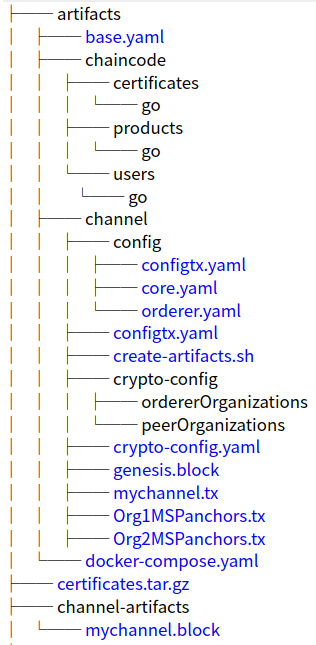
\includegraphics[width = .3 \textwidth]{img/artifacts.png}
    \caption{File structure of the blockchain network}
    \label{fig:networkfilestructure}
\end{figure}

\section{Smart Contracts Design}
% 在Hyper Ledger Fabric中,智能合约被称为链码,本项目的链码使用Golang编写,主要包含处理用户数据和清洁电力证书的智能合约,用户智能合约流程图显示在\fref{fig:flowUser}中,清洁电力证书智能合约流程图由\fref{fig:flowCert}表示。


In Hyper Ledger Fabric, smart contracts are called chain code. The chain code of this project is written in Golang and contains mainly smart contracts for handling user data and clean power certificates. Program flow of the user and clean power certificates contract is shown in \fref{fig:flowUser} and \fref{fig:flowCert}.
\begin{figure}[H]
    \centering
    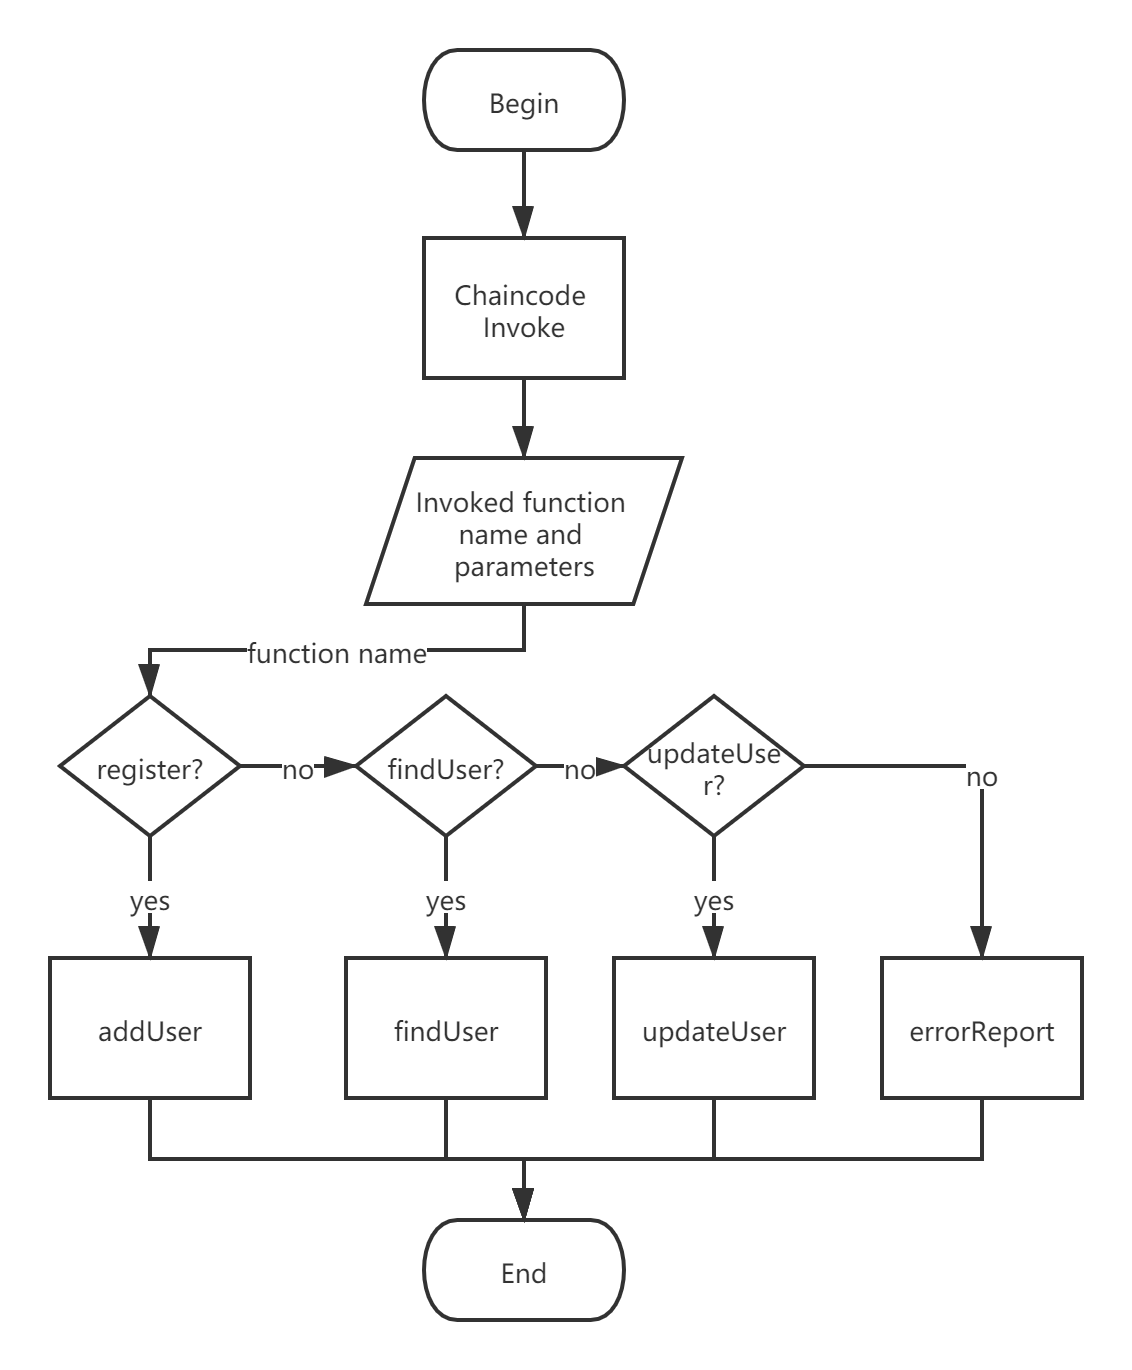
\includegraphics[width=.5 \textwidth]{img/flowUser.png}
    \caption{Program flow of chaincode for users}
    \label{fig:flowUser}
\end{figure}

\begin{figure}[H]
    \centering
    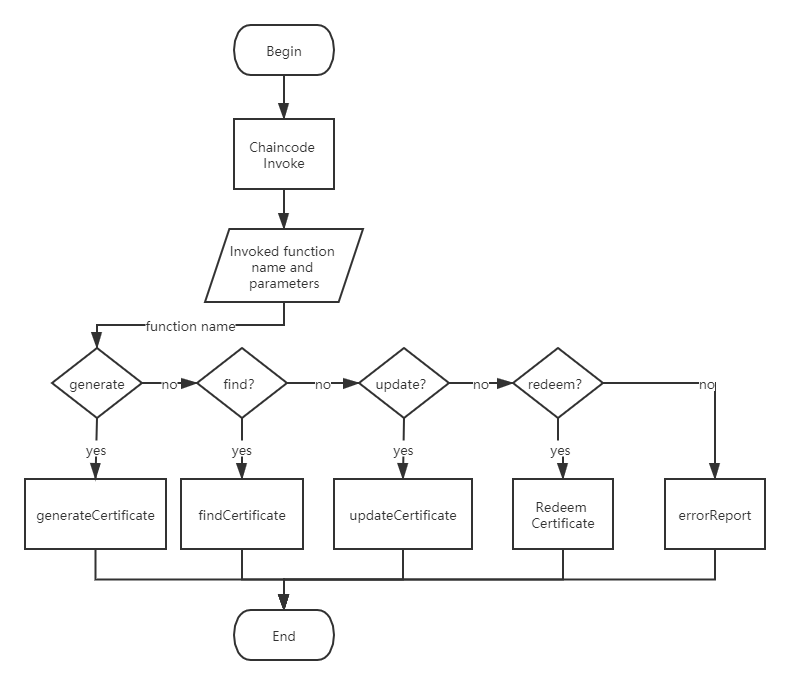
\includegraphics[width=.6 \textwidth]{img/flowCert.png}
    \caption{Program flow of chaincode for clean power certificate}
    \label{fig:flowCert}
\end{figure}

\section{Start Blockchian Network and Deploy Smart Contracts}
% 完成了区块链网络的配置以及智能合约的编写后,就需要开启区块链网络并将智能合约部署到网络中的通道上,通过编写Shell脚本,完成批处理操作后,区块链网络在Docker容器中成功的运行,\fref{fig:dockerps}表示了证书认证节点,排序节点,CouchDB节点以及组织中的四个节点都正常的启动了。
After completing the configuration of the blockchain network and writing the smart contracts, it is time to launch the blockchain network and deploy the smart contracts to the channel in the network. By writing shell scripts and completing batch operations, the blockchain network runs successfully in the Docker container,\fref{fig:dockerps} indicates that the certificate authentication node, the sorting node, the CouchDB node and the four nodes in the organization are started properly.\fref{fig:installchaincode} shows the chaincode has been installed correctly.
\begin{figure}[!htb]
    \centering
    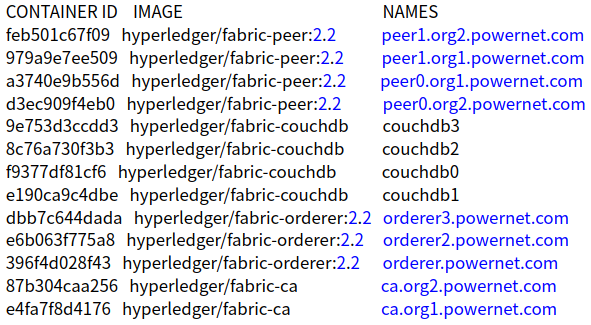
\includegraphics[width=\textwidth]{img/dockerps.png}
    \caption{Docker container process list after starting network}
    \label{fig:dockerps}
\end{figure}

\begin{figure}[!htb]
    \centering
    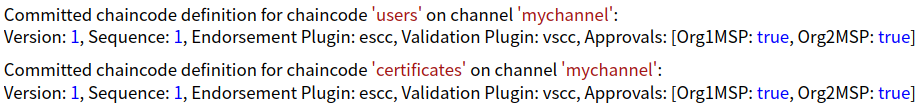
\includegraphics[width=\textwidth]{img/installChaincode.png}
    \caption{Result of installing chaincode}
    \label{fig:installchaincode}
\end{figure}

\section{Coding and realization}
% 智能合约被安装在区块链网络中后,可以将进行UI和后台的开发,实现业务逻辑,本项目使用NodeJS,和React作为实现工具,实现了\fref{fig:login}中的用户登录功能,用户输入邮箱和密码即可登入系统进行操作,也实现了\fref{fig:powermarket},\fref{fig:giftmarket},\fref{fig:pointmarket}中的清洁电力,清洁电力礼品,清洁电力积分交易市场,用户可以在这三个市场进行相应的物品交易,同时还实现了\fref{fig:certmanage}中的清洁能源证书管理功能,可以将清洁能源证书兑换为清洁能点积分。另外的,系统中还实现了用户注册,用户信息管理,订单管理等功能模块没有展现在本文中。
After the smart contract is installed in the blockchain network, the UI and backend development can be carried out to implement the business logic. This project uses NodeJS and React as implementation tools to implement the user login function in \fref{fig:login}, where users can login to the system by entering their email and password, and also implement the clean power, clean power gifts, and clean power points trading markets in \fref{fig:powermarket},\fref{fig:giftmarket}, and \fref{ fig:pointmarket} in the clean power, clean power gifts, clean power points trading market, users can trade the corresponding items in these three markets, and also realized \fref{fig:certmanage} in the clean power certificate management function, can be redeemed clean power certificates for clean power points. In addition, the system also implements user registration, user information management, order management and other functional modules that are not displayed in this paper.
\begin{figure}[!htb]
    \centering
    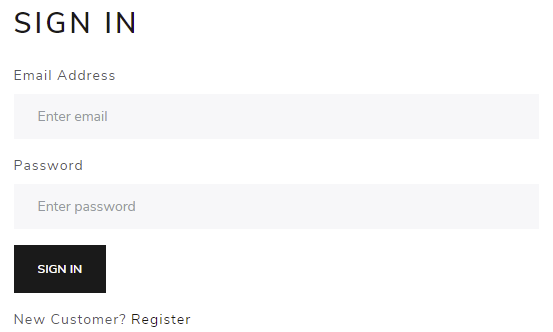
\includegraphics[width=.6 \textwidth]{img/login.png}
    \caption{Login page of the project}
    \label{fig:login}
\end{figure}
\begin{figure}[!htb]
    \centering
    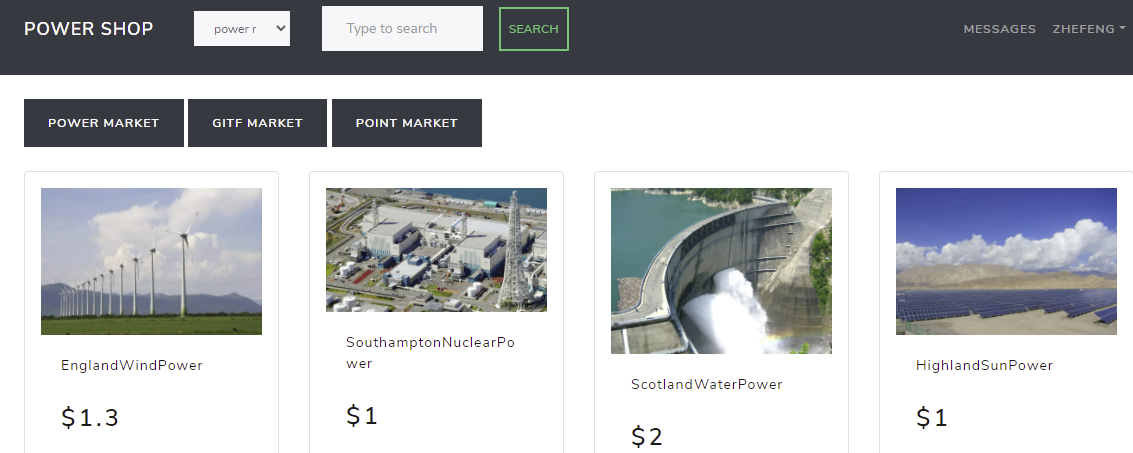
\includegraphics[width= .7\textwidth]{img/powermarket.png}
    \caption{Clean power market of the project}
    \label{fig:powermarket}
\end{figure}
\begin{figure}[!htb]
    \centering
    
\includegraphics[width=.7 \textwidth]{img/giftmarket.png}
    \caption{Clean power market of the project}
    \label{fig:giftmarket}
\end{figure}
\begin{figure}[!htb]
    \centering
    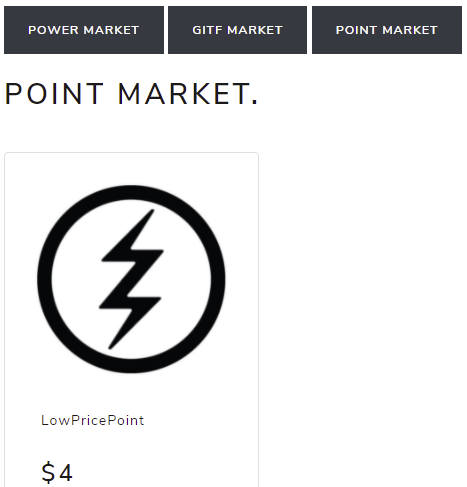
\includegraphics[width= .7 \textwidth]{img/pointmarket.png}
    \caption{Clean power point market of the project}
    \label{fig:pointmarket}
\end{figure}
\begin{figure}[!htb]
    \centering
    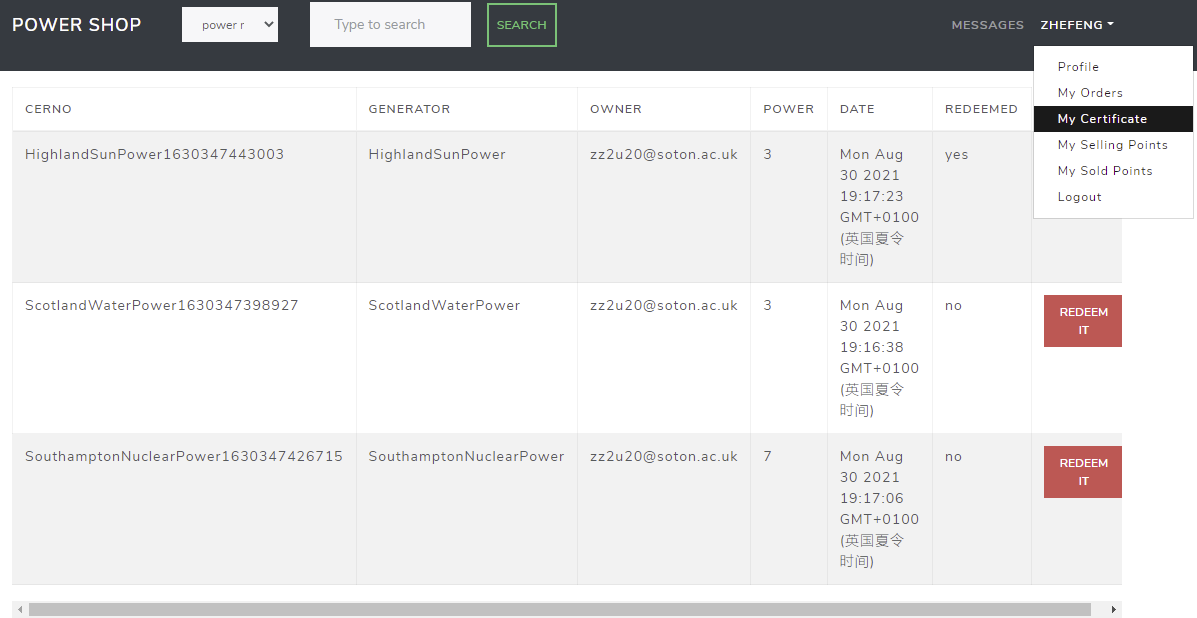
\includegraphics[width=\textwidth]{img/certificateManage.png}
    \caption{Certificates management of the project}
    \label{fig:certmanage}
\end{figure}

